\appendix
    
\chapter{Resultados del Benchmark en Entorno Local (Compu Juan)}
\label{appendix:local}
En este anexo se presentan las tablas de tiempos, speedup y eficiencia obtenidos en el entorno local. 

\begin{figure}[H]
    \centering
    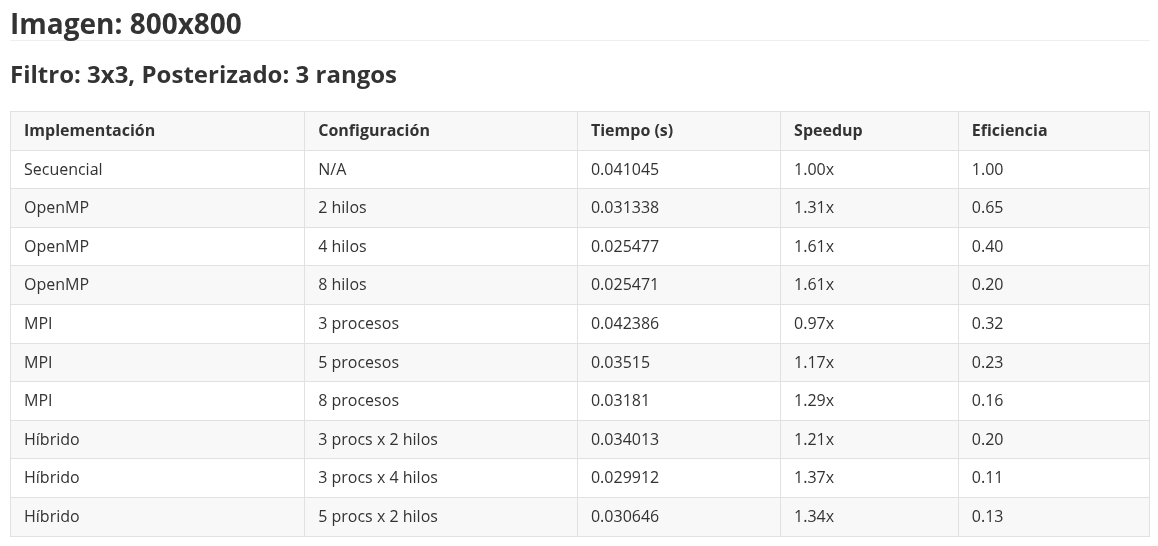
\includegraphics[width=1\textwidth]{resources/800local3x33.png}
    \caption{Resultados del benchmark en entorno local para imagen de 800x800, kernel 3x3 y 3 rangos de posterización.}
    \label{fig:800_local_3x3_3}
\end{figure}


\begin{figure}[H]
    \centering
    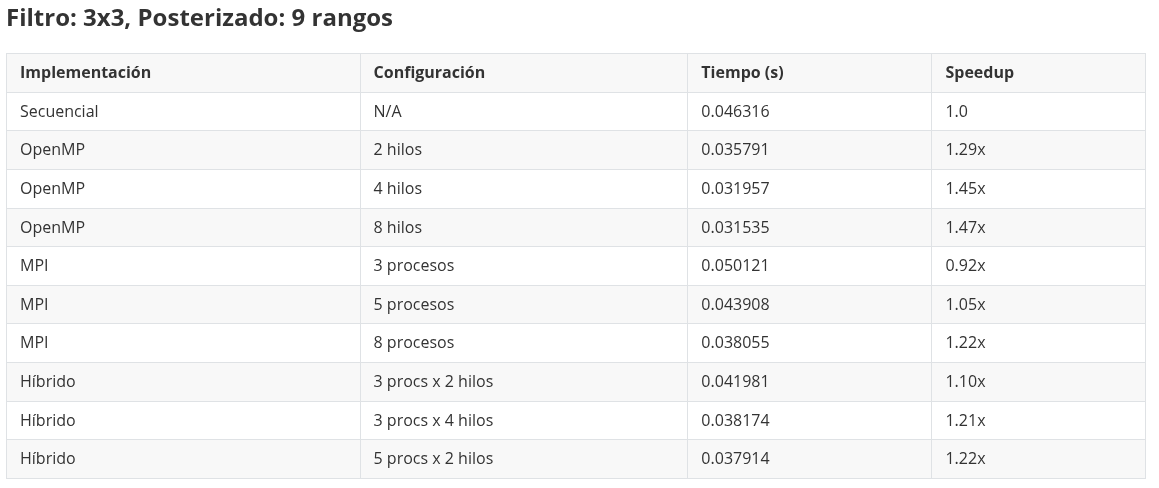
\includegraphics[width=1\textwidth]{resources/800local3x39.png}
    \caption{Resultados del benchmark en entorno local para imagen de 800x800, kernel 3x3 y 9 rangos de posterización.}
    \label{fig:800_local_3x3_9}
\end{figure}

\begin{figure}[H]
    \centering
    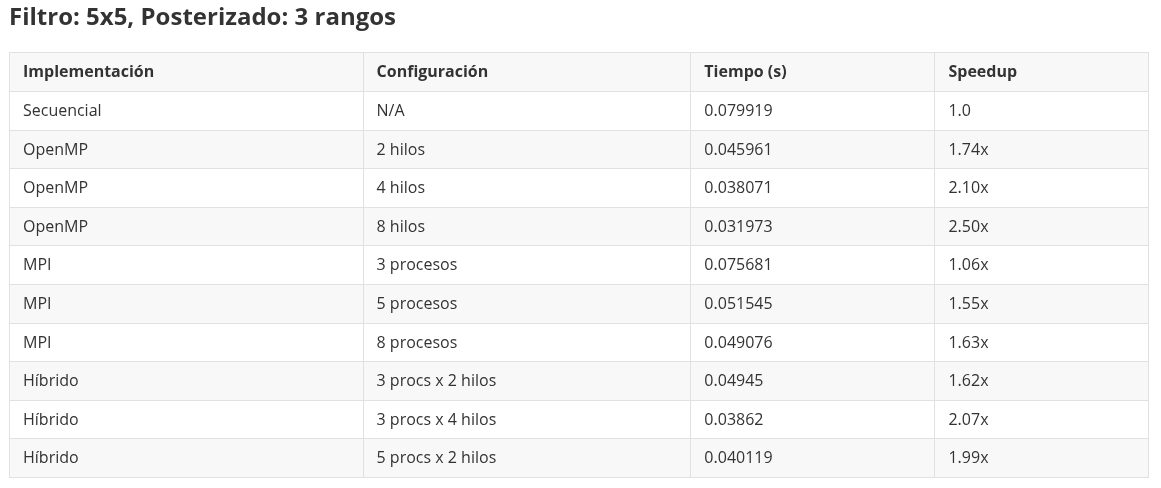
\includegraphics[width=1\textwidth]{resources/800local5x53.png}
    \caption{Resultados del benchmark en entorno local para imagen de 800x800, kernel 5x5 y 3 rangos de posterización.}
    \label{fig:800_local_5x5_3}
\end{figure}


\begin{figure}[H]
    \centering
    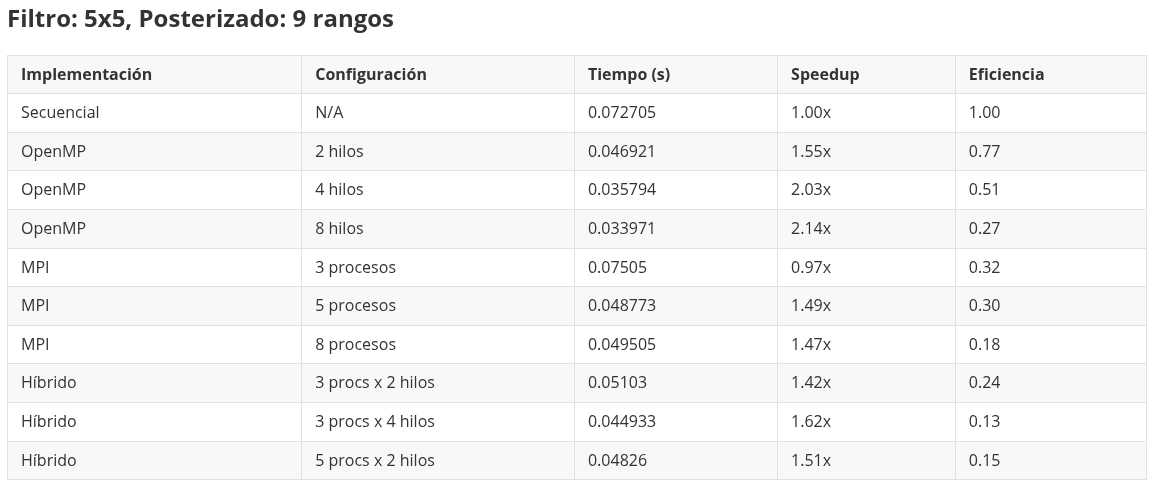
\includegraphics[width=1\textwidth]{resources/800local5x59.png}
    \caption{Resultados del benchmark en entorno local para imagen de 800x800, kernel 5x5 y 9 rangos de posterización.}
    \label{fig:800_local_5x5_9}
\end{figure}

% -------------------------------------------------------------------

\begin{figure}[H]
    \centering
    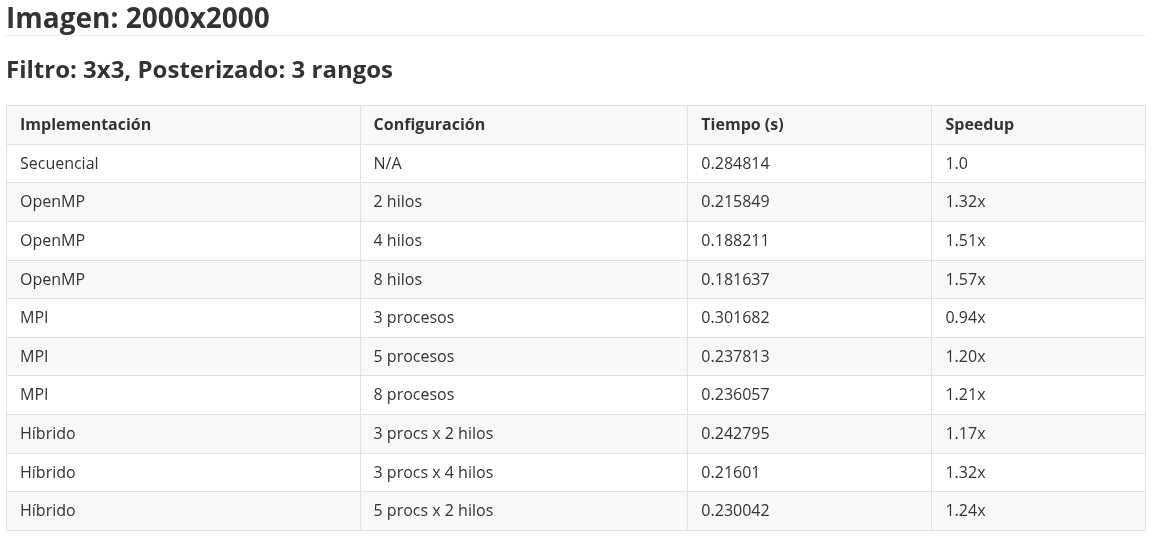
\includegraphics[width=1\textwidth]{resources/2000local3x33.png}
    \caption{Resultados del benchmark en entorno local para imagen de 2000x2000, kernel 3x3 y 3 rangos de posterización.}
    \label{fig:2000_local_3x3_3}
\end{figure}


\begin{figure}[H]
    \centering
    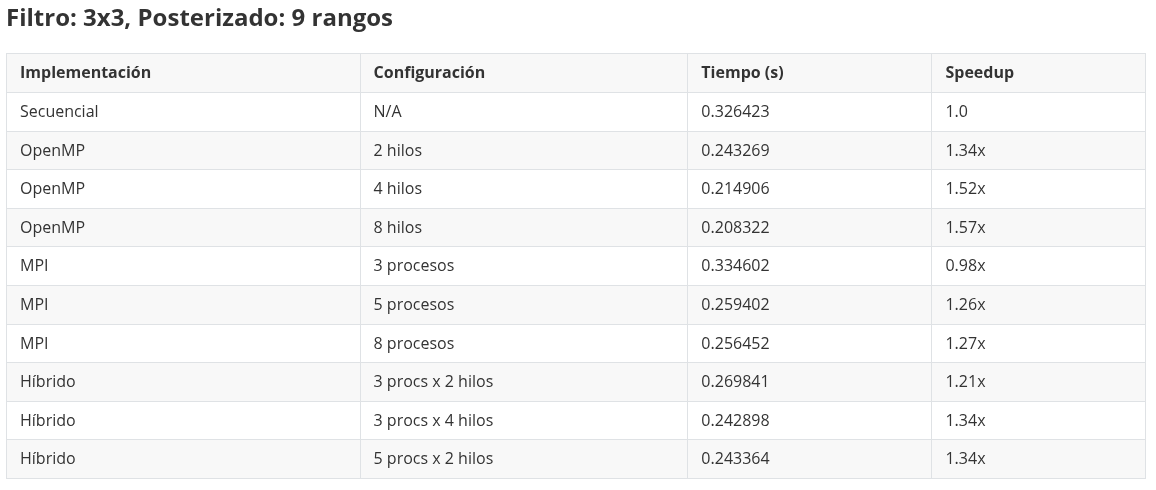
\includegraphics[width=1\textwidth]{resources/2000local3x39.png}
    \caption{Resultados del benchmark en entorno local para imagen de 2000x2000, kernel 3x3 y 9 rangos de posterización.}
    \label{fig:2000_local_3x3_9}
\end{figure}

\begin{figure}[H]
    \centering
    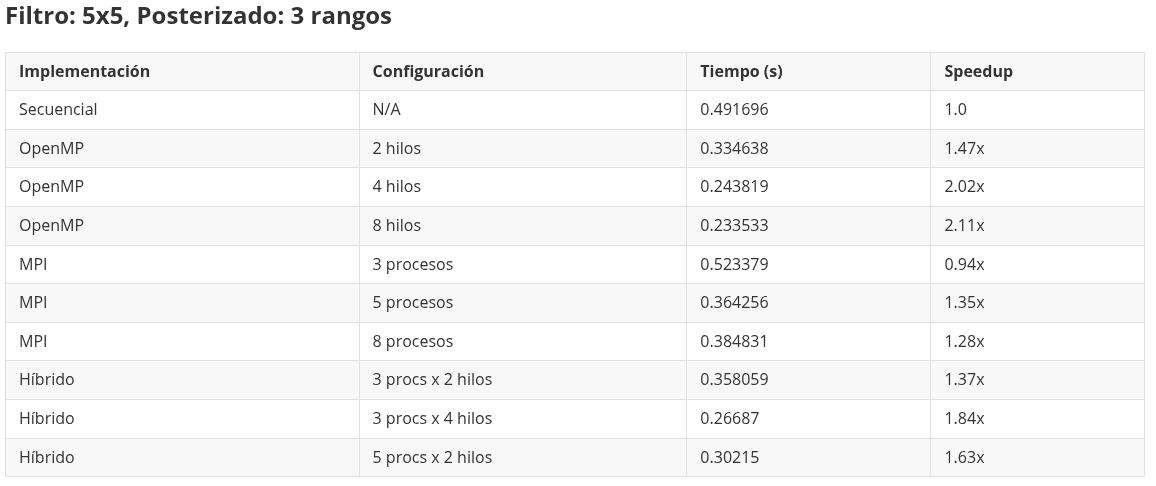
\includegraphics[width=1\textwidth]{resources/2000local5x53.png}
    \caption{Resultados del benchmark en entorno local para imagen de 2000x2000, kernel 5x5 y 3 rangos de posterización.}
    \label{fig:2000_local_5x5_3}
\end{figure}


\begin{figure}[H]
    \centering
    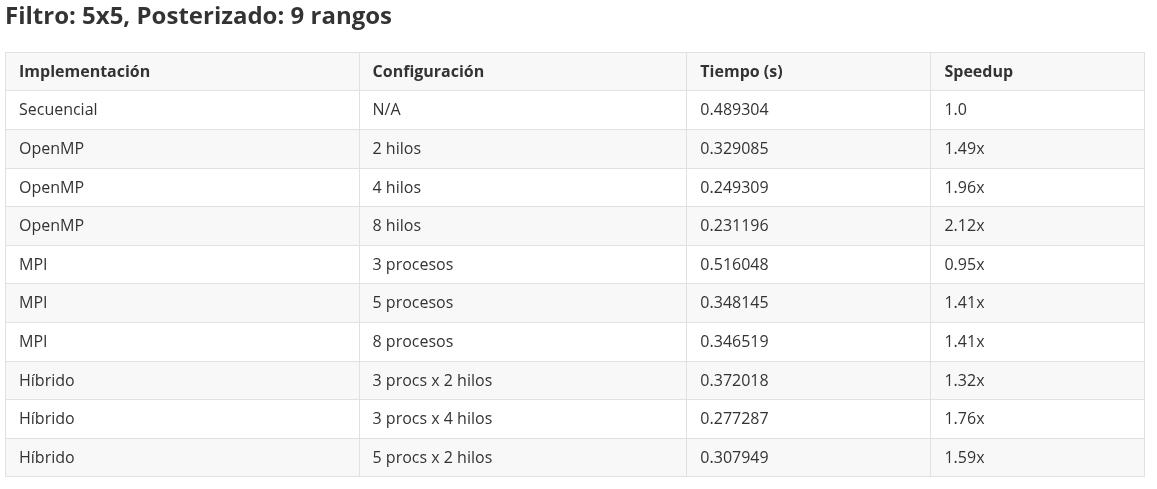
\includegraphics[width=1\textwidth]{resources/2000local5x59.png}
    \caption{Resultados del benchmark en entorno local para imagen de 2000x2000, kernel 5x5 y 9 rangos de posterización.}
    \label{fig:2000_local_5x5_9}
\end{figure}

% -------------------------------------------------------------------

\begin{figure}[H]
    \centering
    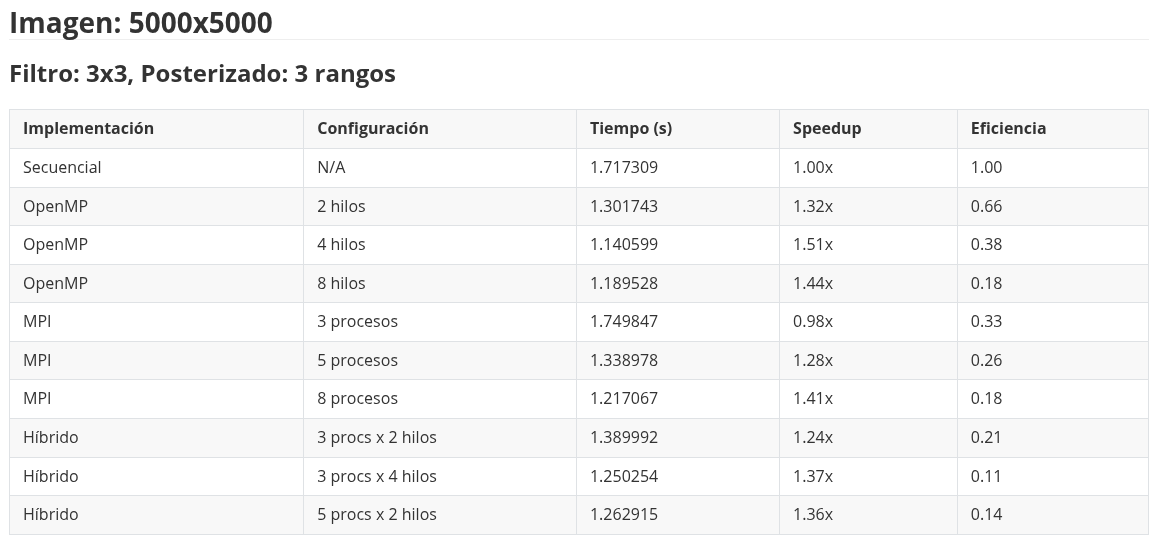
\includegraphics[width=1\textwidth]{resources/5000local3x33.png}
    \caption{Resultados del benchmark en entorno local para imagen de 5000x5000, kernel 3x3 y 3 rangos de posterización.}
    \label{fig:5000_local_3x3_3}
\end{figure}


\begin{figure}[H]
    \centering
    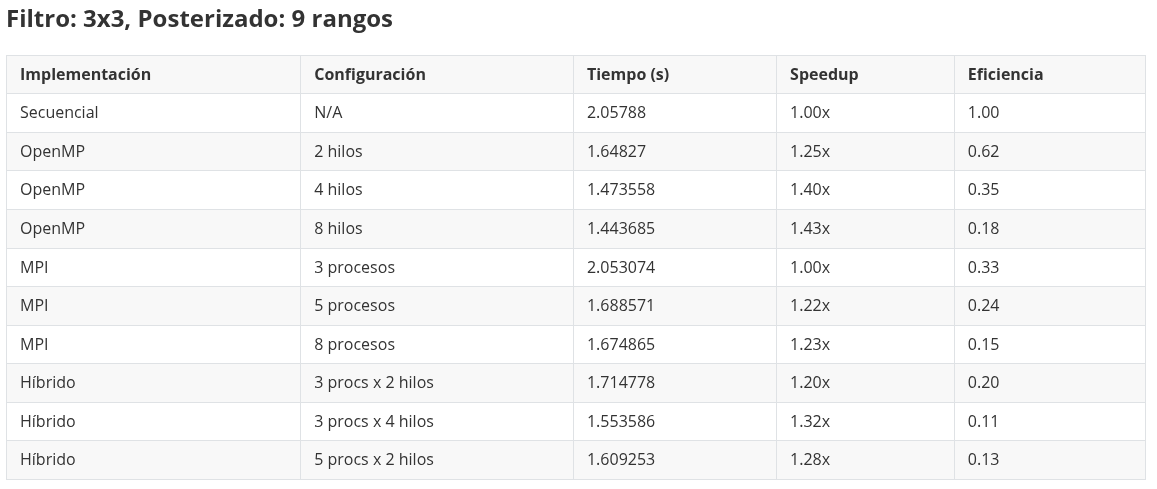
\includegraphics[width=1\textwidth]{resources/5000local3x39.png}
    \caption{Resultados del benchmark en entorno local para imagen de 5000x5000, kernel 3x3 y 9 rangos de posterización.}
    \label{fig:5000_local_3x3_9}
\end{figure}

\begin{figure}[H]
    \centering
    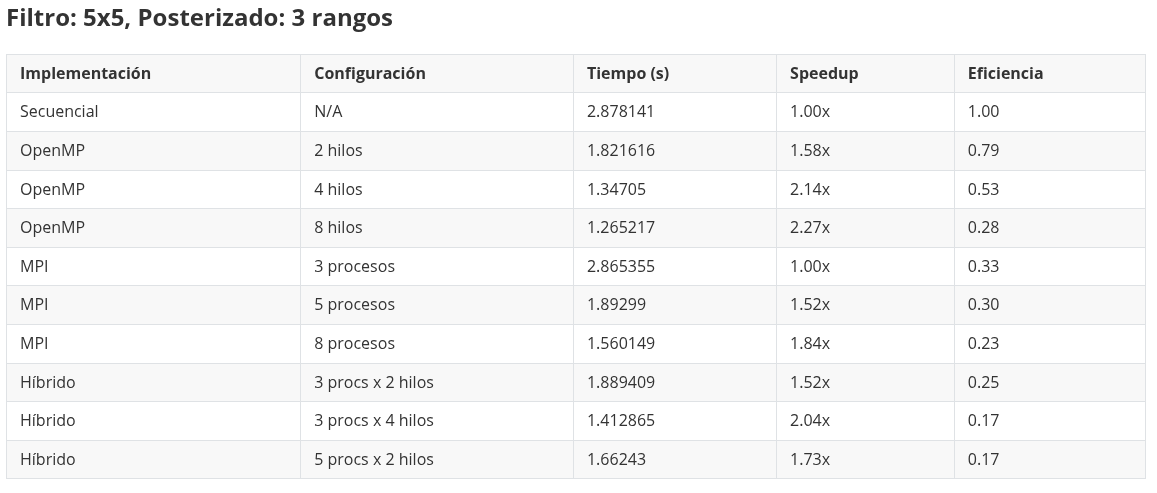
\includegraphics[width=1\textwidth]{resources/5000local5x53.png}
    \caption{Resultados del benchmark en entorno local para imagen de 5000x5000, kernel 5x5 y 3 rangos de posterización.}
    \label{fig:5000_local_5x5_3}
\end{figure}


\begin{figure}[H]
    \centering
    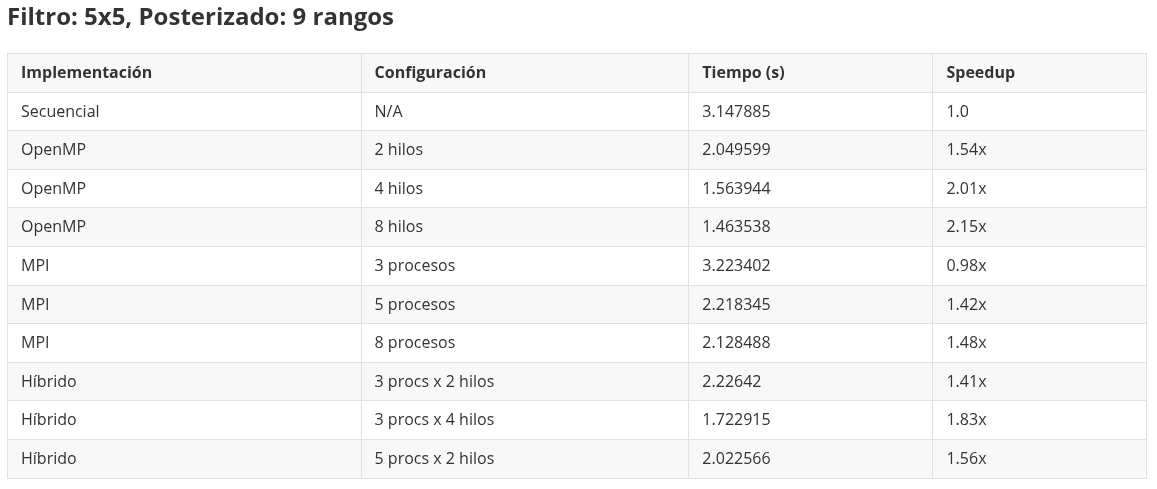
\includegraphics[width=1\textwidth]{resources/5000local5x59.png}
    \caption{Resultados del benchmark en entorno local para imagen de 5000x5000, kernel 5x5 y 9 rangos de posterización.}
    \label{fig:5000_local_5x5_9}
\end{figure}

% -------------------------------------------------------------------

\chapter{Resultados del Benchmark en Entorno Cluster (Ejecución 2)}
\label{appendix:cluster}
En este anexo se presentan las tablas de tiempos, speedup y eficiencia obtenidos en el cluster del Departamento. 

% -------------------------------------------------------------------

\begin{figure}[H]
    \centering
    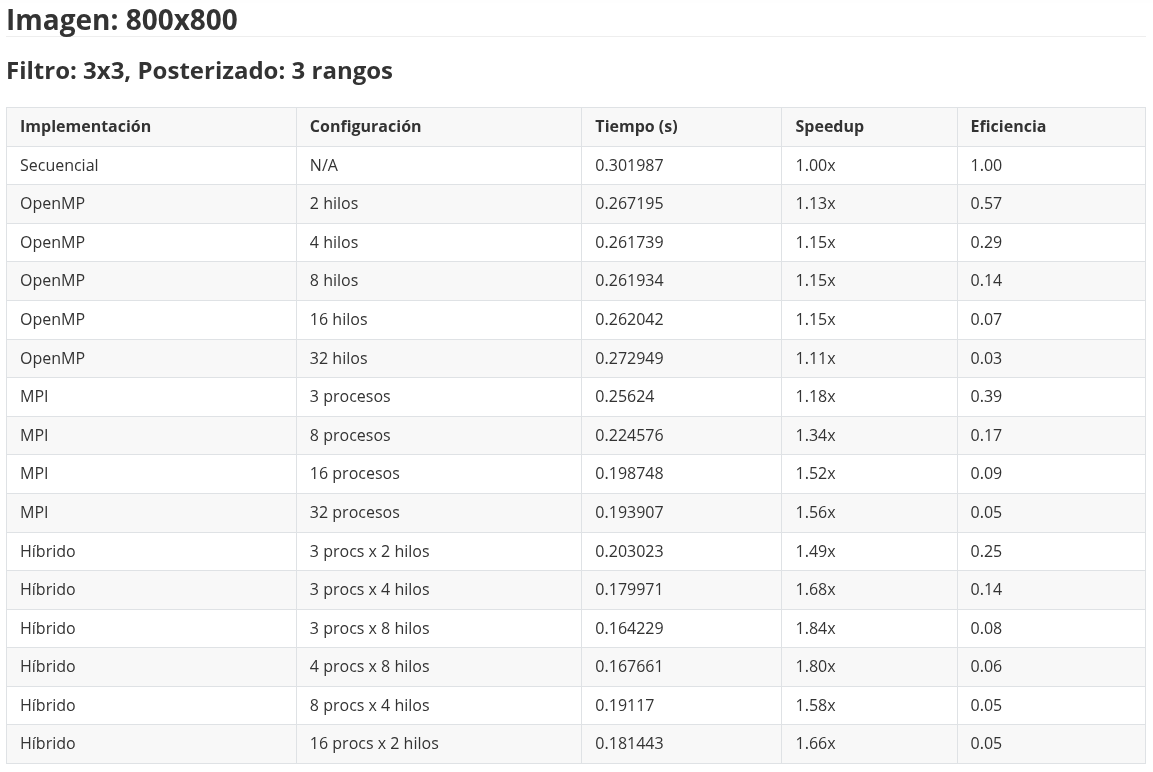
\includegraphics[width=1\textwidth]{resources/800cluster3x33.png}
    \caption{Resultados del benchmark en entorno cluster para imagen de 800x800, kernel 3x3 y 3 rangos de posterización.}
    \label{fig:800_cluster_3x3_3}
\end{figure}


\begin{figure}[H]
    \centering
    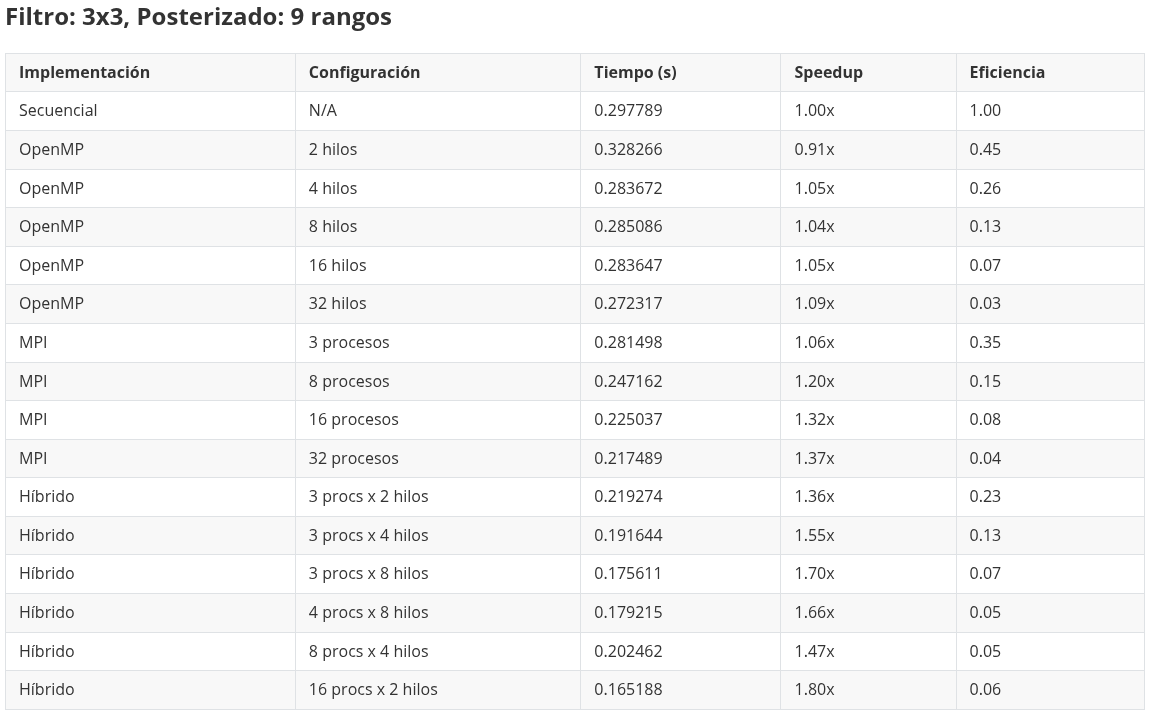
\includegraphics[width=1\textwidth]{resources/800cluster3x39.png}
    \caption{Resultados del benchmark en entorno cluster para imagen de 800x800, kernel 3x3 y 9 rangos de posterización.}
    \label{fig:800_cluster_3x3_9}
\end{figure}

\begin{figure}[H]
    \centering
    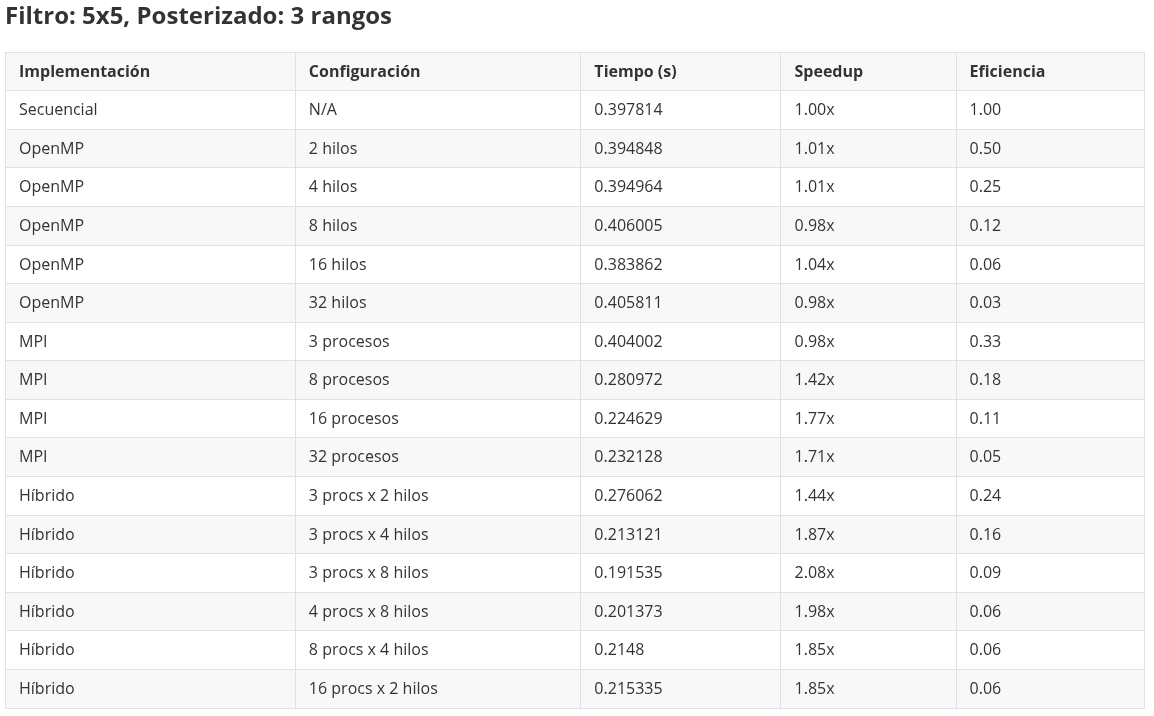
\includegraphics[width=1\textwidth]{resources/800cluster5x53.png}
    \caption{Resultados del benchmark en entorno cluster para imagen de 800x800, kernel 5x5 y 3 rangos de posterización.}
    \label{fig:800_cluster_5x5_3}
\end{figure}


\begin{figure}[H]
    \centering
    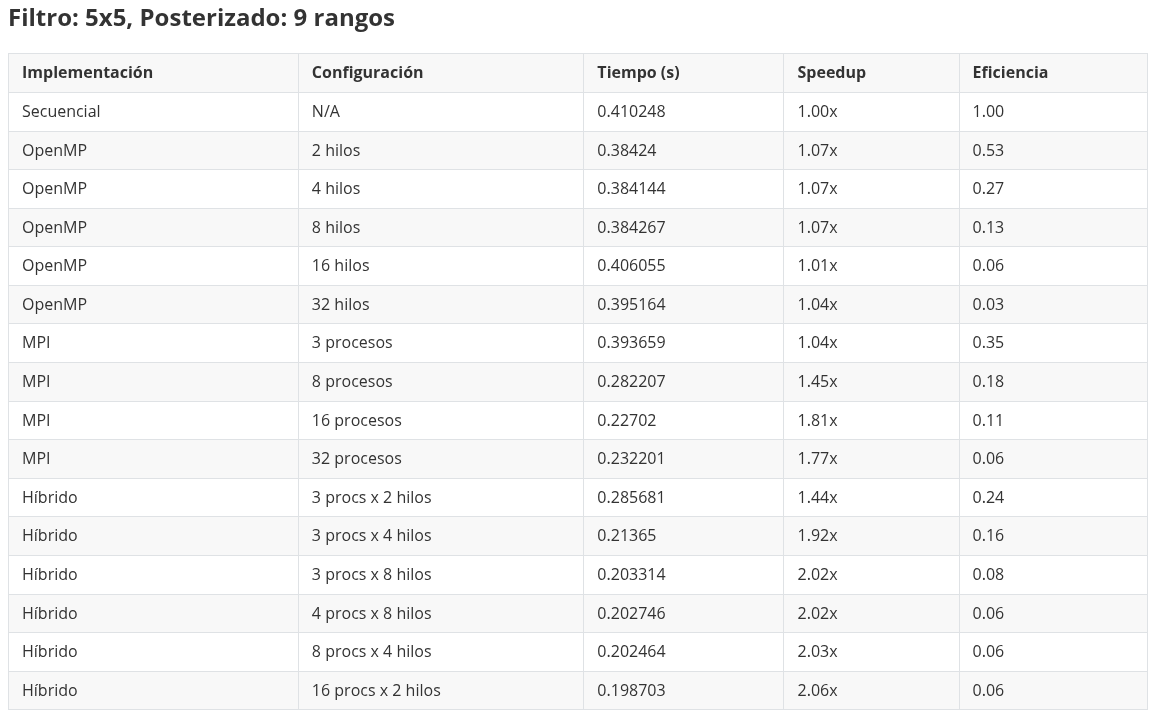
\includegraphics[width=1\textwidth]{resources/800cluster5x59.png}
    \caption{Resultados del benchmark en entorno cluster para imagen de 800x800, kernel 5x5 y 9 rangos de posterización.}
    \label{fig:800_cluster_5x5_9}
\end{figure}

% -------------------------------------------------------------------

\begin{figure}[H]
    \centering
    \includegraphics[width=1\textwidth]{resources/2000cluster3x33.png}
    \caption{Resultados del benchmark en entorno cluster para imagen de 2000x2000, kernel 3x3 y 3 rangos de posterización.}
    \label{fig:2000_cluster_3x3_3}
\end{figure}


\begin{figure}[H]
    \centering
    \includegraphics[width=1\textwidth]{resources/2000cluster3x39.png}
    \caption{Resultados del benchmark en entorno cluster para imagen de 2000x2000, kernel 3x3 y 9 rangos de posterización.}
    \label{fig:2000_cluster_3x3_9}
\end{figure}

\begin{figure}[H]
    \centering
    \includegraphics[width=1\textwidth]{resources/2000cluster5x53.png}
    \caption{Resultados del benchmark en entorno cluster para imagen de 2000x2000, kernel 5x5 y 3 rangos de posterización.}
    \label{fig:2000_cluster_5x5_3}
\end{figure}


\begin{figure}[H]
    \centering
    \includegraphics[width=1\textwidth]{resources/2000cluster5x59.png}
    \caption{Resultados del benchmark en entorno cluster para imagen de 2000x2000, kernel 5x5 y 9 rangos de posterización.}
    \label{fig:2000_cluster_5x5_9}
\end{figure}

% -------------------------------------------------------------------

\begin{figure}[H]
    \centering
    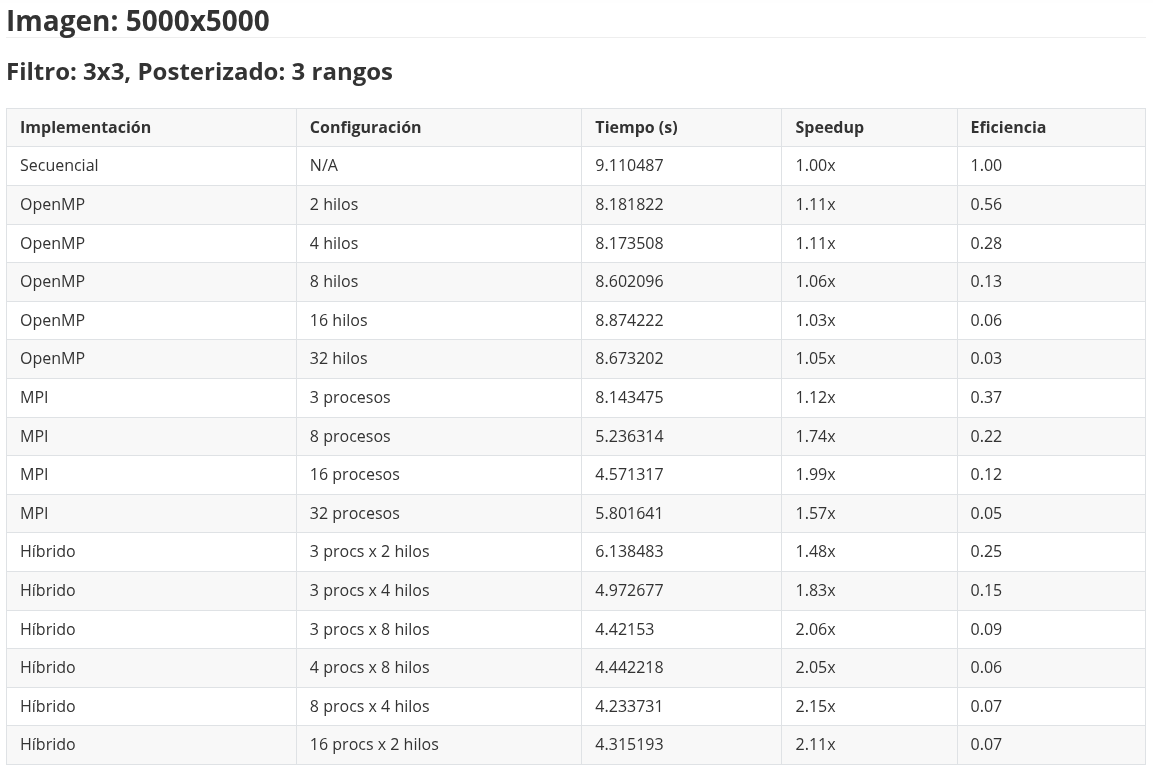
\includegraphics[width=1\textwidth]{resources/5000cluster3x33.png}
    \caption{Resultados del benchmark en entorno cluster para imagen de 5000x5000, kernel 3x3 y 3 rangos de posterización.}
    \label{fig:5000_cluster_3x3_3}
\end{figure}


\begin{figure}[H]
    \centering
    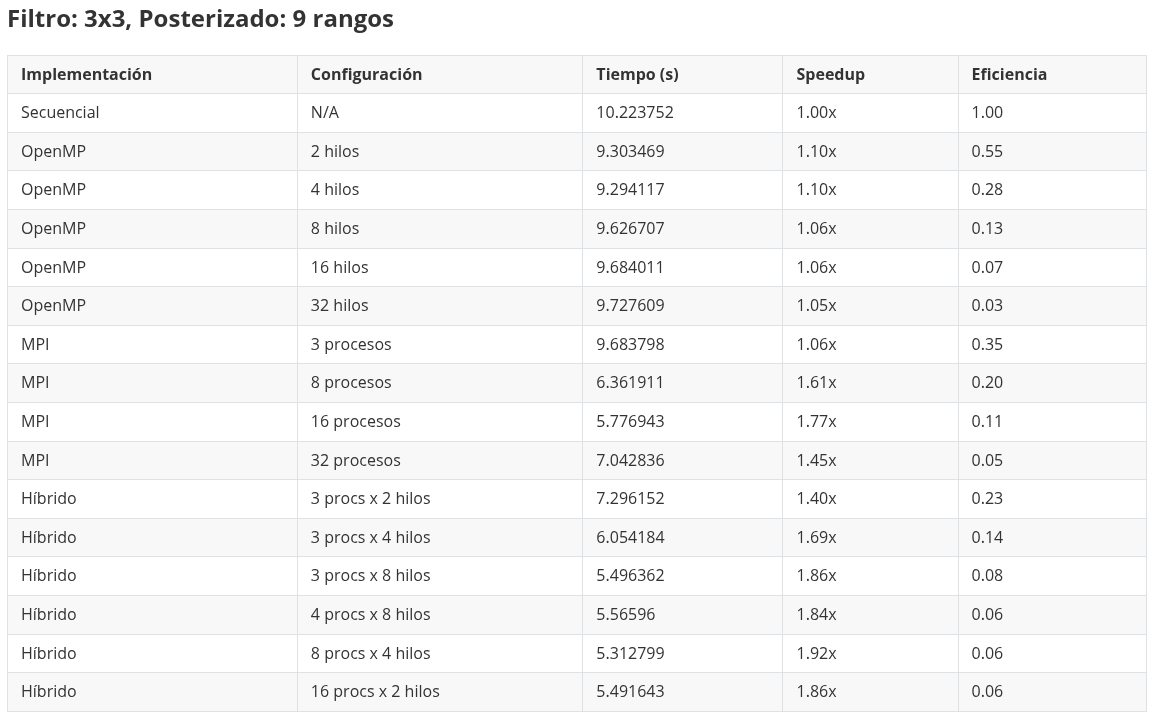
\includegraphics[width=1\textwidth]{resources/5000cluster3x39.png}
    \caption{Resultados del benchmark en entorno cluster para imagen de 5000x5000, kernel 3x3 y 9 rangos de posterización.}
    \label{fig:5000_cluster_3x3_9}
\end{figure}

\begin{figure}[H]
    \centering
    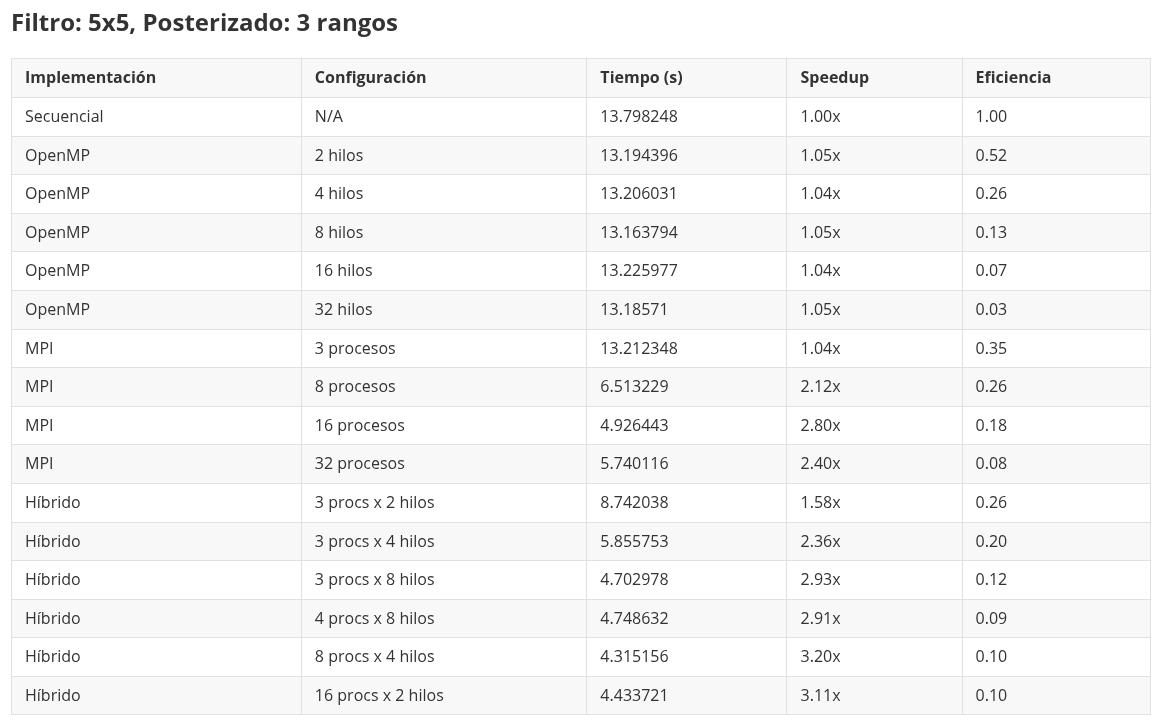
\includegraphics[width=1\textwidth]{resources/5000cluster5x53.png}
    \caption{Resultados del benchmark en entorno cluster para imagen de 5000x5000, kernel 5x5 y 3 rangos de posterización.}
    \label{fig:5000_cluster_5x5_3}
\end{figure}


\begin{figure}[H]
    \centering
    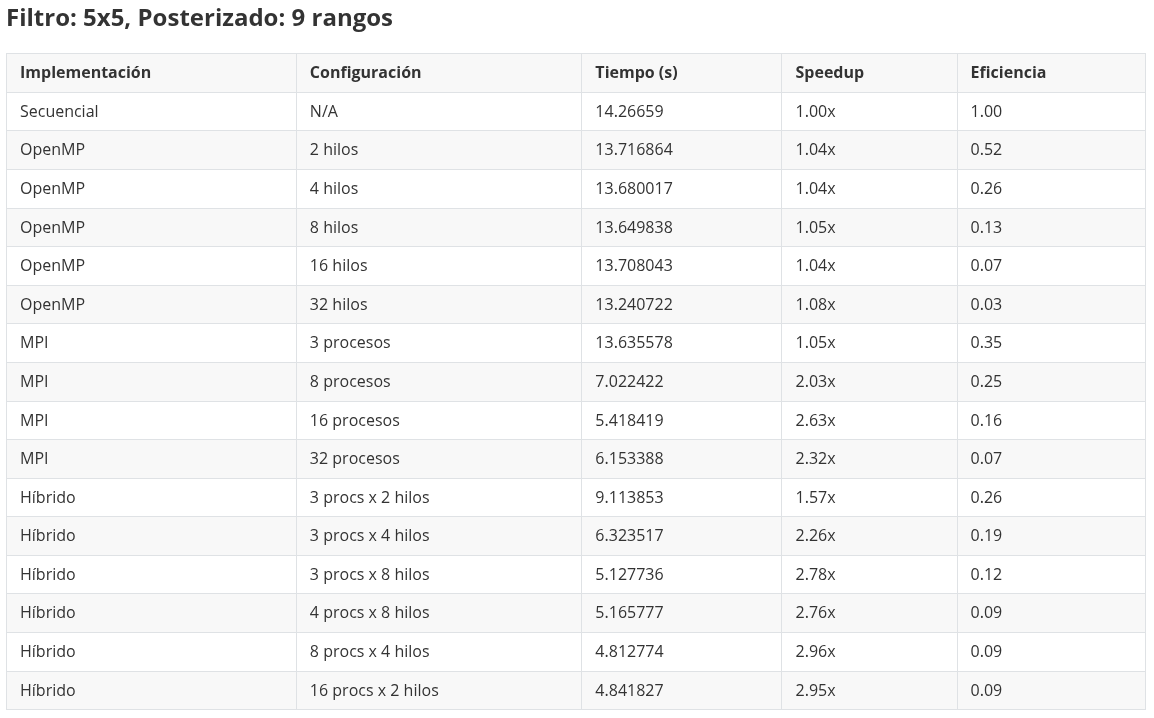
\includegraphics[width=1\textwidth]{resources/5000cluster5x59.png}
    \caption{Resultados del benchmark en entorno cluster para imagen de 5000x5000, kernel 5x5 y 9 rangos de posterización.}
    \label{fig:5000_cluster_5x5_9}
\end{figure}